\part{Windows}
\setcounter{section}{0}
\clearpage
\section{压缩刻录}


\section{聊天工具}
\section{视频软件}
\section{音乐软件}
\section{游戏软件}
\section{网络游戏}
\section{浏览器}
\section{图形图像}
\section{输入法}
\section{下载工具}
\section{办公软件}
\section{阅读翻译}
\clearpage
\section{系统工具}
\subsection{lmtghost3.0.exe-备份还原操作系统}
准备工作
\begin{itemize}
\item 备份还原软件--\href{http://ghost.laomaotao.net/help/330/}{老毛桃一键还原}
\end{itemize} 
操作步骤
\begin{itemize}
\item 备份系统
\begin{enumerate}
\item 主程序兼容Win2003、Winxp、Win7以及WinPE系统。为避免部分杀毒软件误报,请尽量在运行程序前退出杀软或在安全类软件提示是否允许操作时信任本程序运行。初次运行程序会提示进行初始备份,点击一键备份系统按钮后根据程序提示选择重新启动。\\
\begin{figure}[!htbp]
	\centering
	\caption{备份参数设置}  
		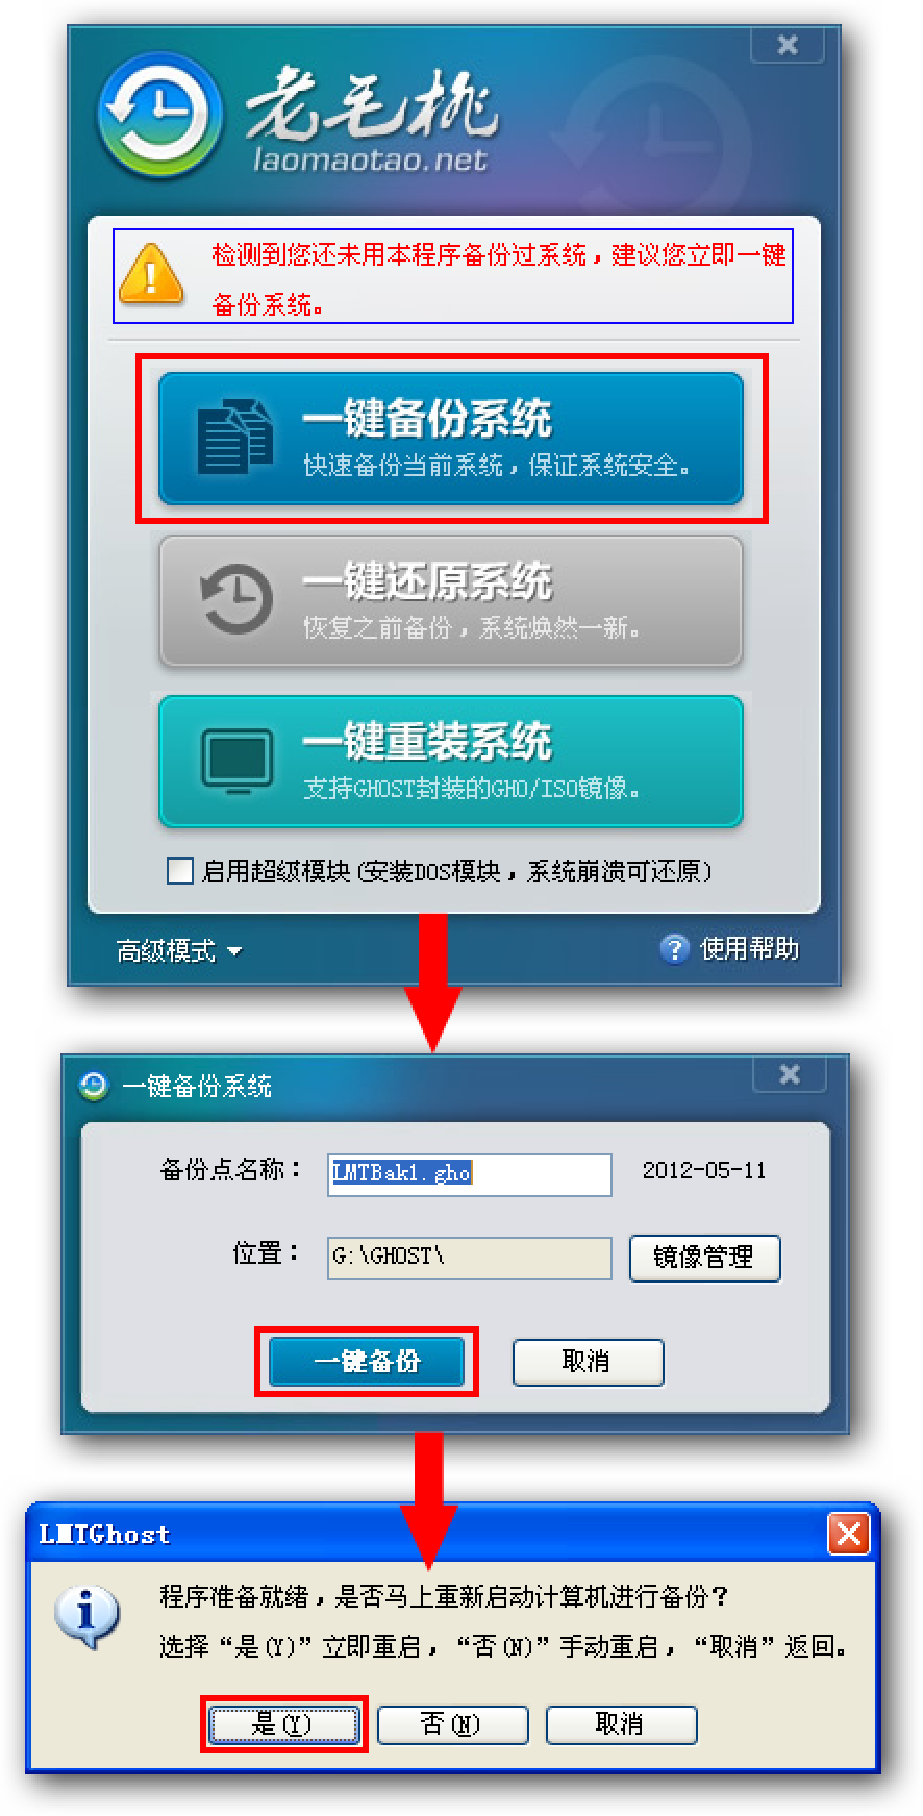
\includegraphics[scale=0.40]{figs/win_lmt_backup_startup.pdf}
    	\label{fig:win_lmt_backup_startup}
\end{figure}

\item 重新启动电脑后会自动进入老毛桃一键还原界面进行自动系统备份。\\
\begin{figure}[!htbp]
	\centering
	\caption{备份过程}  
		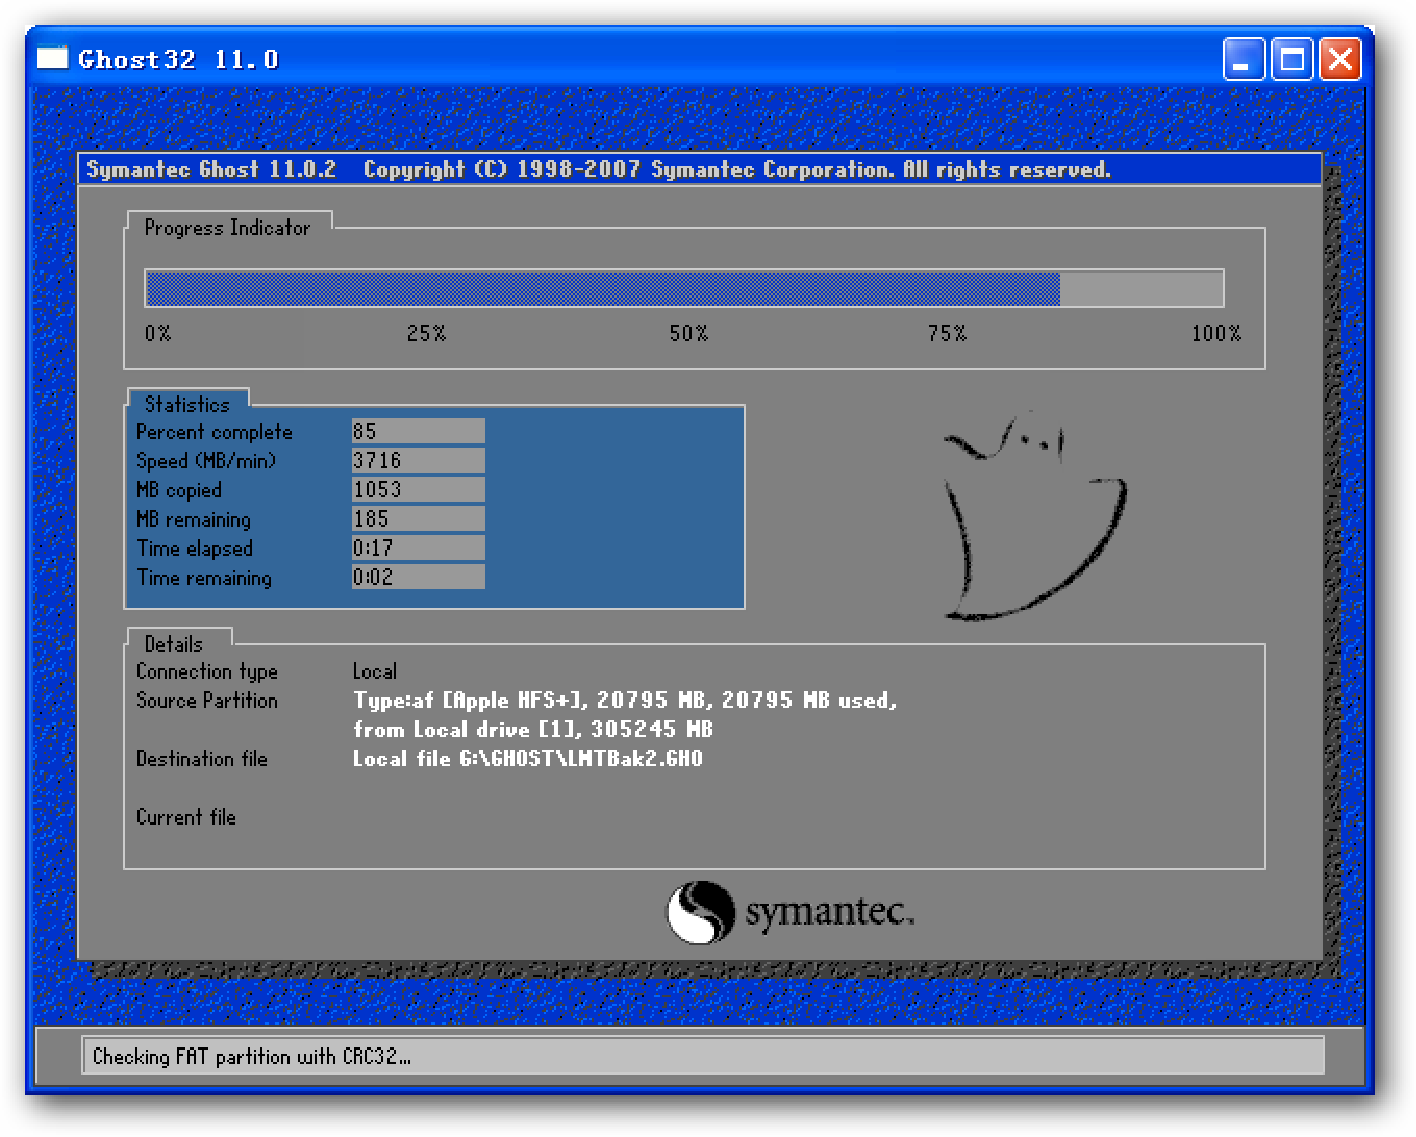
\includegraphics[scale=0.35]{figs/win_lmt_backup_set.pdf}
    	\label{fig:win_lmt_backup_set}
\end{figure}

\end{enumerate}

\item 还原系统\\
\begin{enumerate}
\item 备份完毕后重新启动电脑,打开老毛桃一键还原程序即可看到程序自动检测到刚刚备份了系统。以后当系统中毒或是出现其它问题时点击\textcolor{red}{(请在还原之前提前备份好系统盘的个人资料,还原时将对C盘原有数据进行覆盖)}。即可将系统恢复到之前备份的状态。\\
\begin{figure}[!htbp]
	\centering
	\caption{还原设置}  
		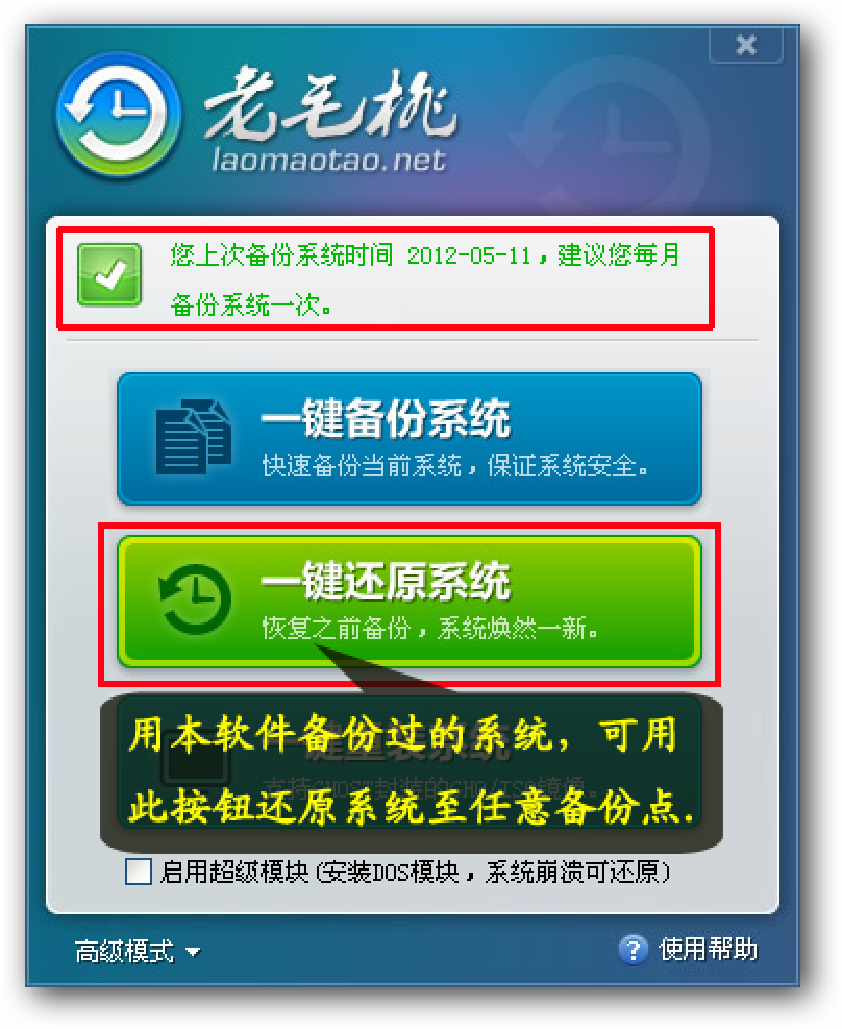
\includegraphics[scale=0.35]{figs/win_lmt_restore_startup.pdf}
    	\label{fig:win_lmt_backup_result}
\end{figure}
\end{enumerate}

\item 重装系统\\
\begin{enumerate}
\item 如果没有执行过系统备份想要重新安装系统,可以使用一键重装功能全新安装系统。一键重装系统功能支持GHOST封装的GHO/ISO镜像。\\
\begin{figure}[!htbp]
	\centering
	\caption{重装系统}  
		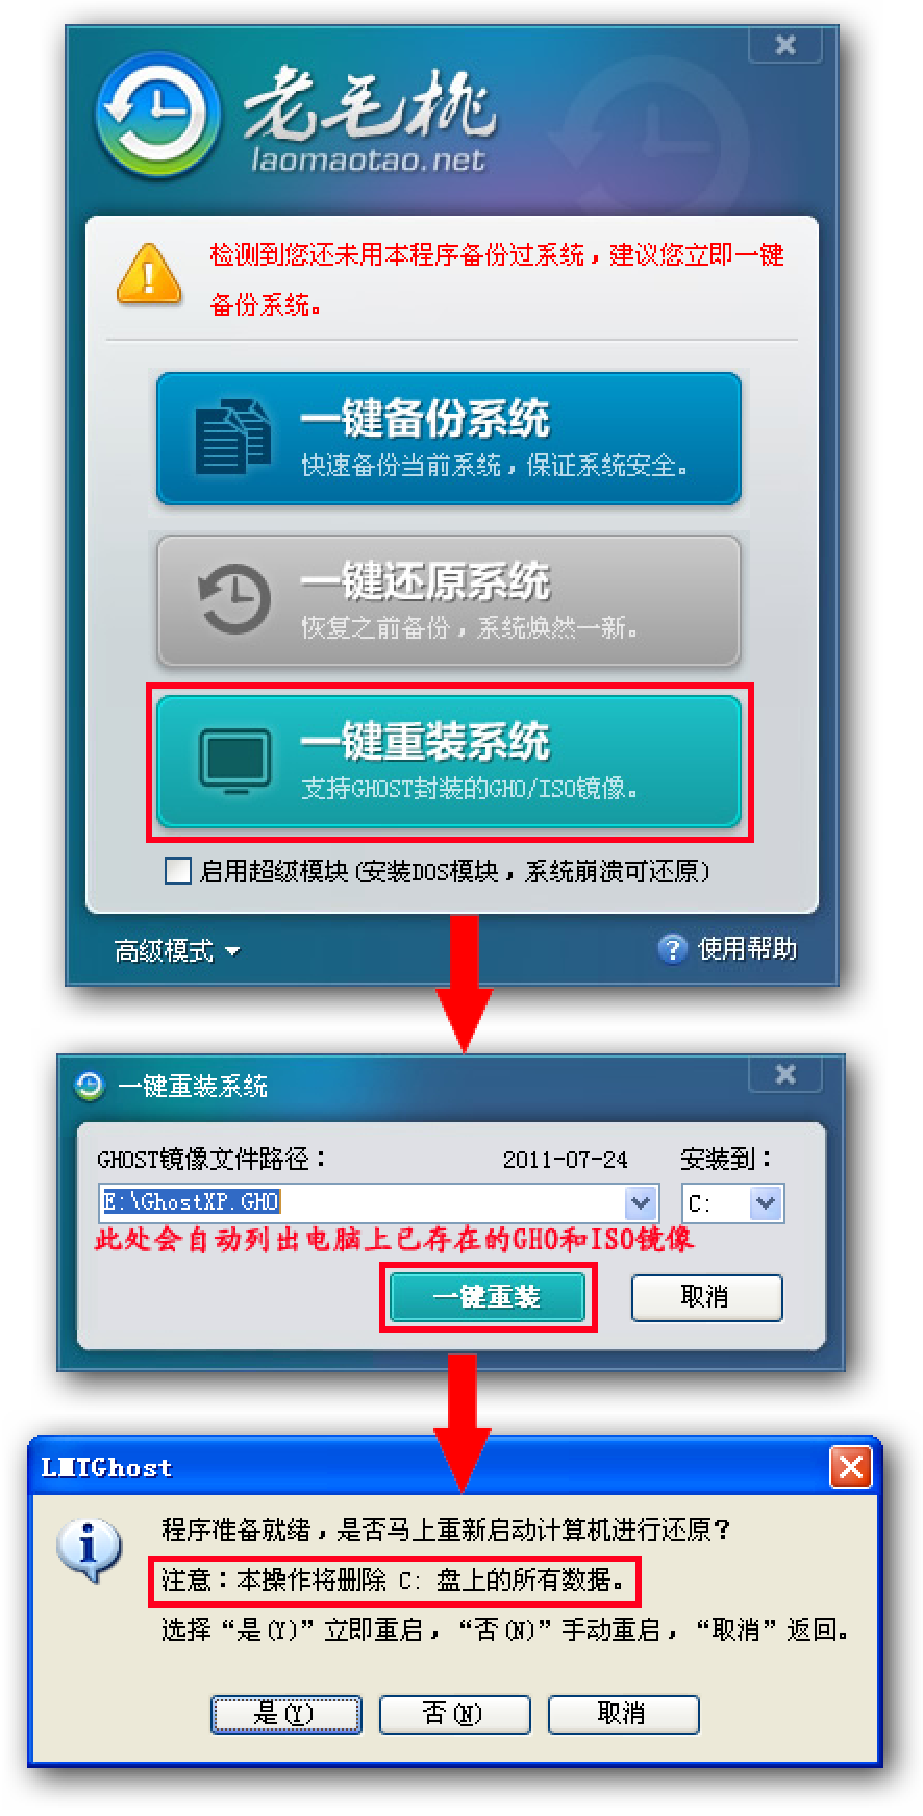
\includegraphics[scale=0.35]{figs/win_lmt_reinstall_startup.pdf}
    	\label{fig:win_lmt_backup_result}
\end{figure}
\end{enumerate}

\end{itemize}
\clearpage
\section{编程开发}
\clearpage
\section{其他软件}
\subsection{ubuntu one-网盘}
背景介绍\\

Ubuntu One是由Ubuntu背后的公司Canonical所推出的一项网络服务。该服务能够存储你的文件,并允许你在多台电脑上同步,还可以与好友分享这些文件。\\
准备工作
\begin{itemize}
\item 帐号--\href{https://one.ubuntu.com/dashboard}{ubuntu one官网}
\item 软件--\href{https://one.ubuntu.com/downloads/windows/}{Ubuntu One}
\end{itemize} 
优势总结
\begin{description}
\item[跨平台] 目前的客户端支持windows,ubuntu,mac,android和iphone
\item[容量] 免费5G,\$2.99/月即可获得20G。
\item[速度] 同步速度大约在80kb/s,更重要的是同步响应非常快。
\item[共享] 指定欲分享用户的Email地址既可分享文件夹,发送链接既可分享指定文件。
\end{description}
使用推荐:\textcolor{red}{存储私人关键文件}

\subsection{google driver-网盘}
背景介绍\\

Google Drive,美国谷歌公司于2012年4月24日正式推出的一项云存储服务,可以向用户提供5GB的免费存储空间,同时还可以付费扩容。\\
准备工作
\begin{itemize}
\item google帐号--\href{https://accounts.google.com/SignUp?hl=zh-CN}{帐号注册}
\item 软件--\href{http://drive.google.com}{云端硬盘}
\end{itemize} 
优势总结
\begin{description}
\item[跨平台] 目前的客户端支持windows,mac,android和ubuntu(有适用期)
\item[容量] 免费5G,\$2.49/月即可获得25G。
\item[在线浏览] 支持多达30多种文件的直接预览。
\item[集中管理] 对于文件的管理非常方便。
\end{description}
使用推荐:\textcolor{red}{作为公开网盘,用来存储文档以及常用软件}


\subsection{dropbox-网盘}
背景介绍\\

Dropbox是一个提供同步本地文件的网络存储在线应用。支持在多台电脑多种操作中自动同步。并可当作大容量的网络硬盘使用。\\
准备工作
\begin{itemize}
\item 帐号--\href{https://www.dropbox.com/}{dropbox官网}
\item 软件--\href{http://dropboxchina.com/Download/dropbox-for-windows.html}{dropbox}
\end{itemize} 
优势总结
\begin{description}
\item[跨平台] 目前的客户端支持windows,ubuntu,mac,android,iphone和blackberry
\item[容量] 免费3G,通过邀请朋友可获得额外空间。
\item[图片预览] 支持图片直接预览。
\item[国外流行] 成为很多软件首选的备份点,如springseed。
\end{description}
使用推荐:\textcolor{red}{配合android版备份手机上的照片}


\clearpage
\section{安全杀毒}
\clearpage














